\chapter{Interfejs}
\label{cha:interfejs}

Interfejs aplikacji składa się z trzech rodzielnych zbiorów ekranów. Każda nawigacja pomiędzy tymi grupami skutkuje usunięciem z pamięci kolekcji ekranów, znajdujących się w poprzedniej grupie oraz załadowaniem nowego zestawu.
W pierwszym pakiecie znajdują ekrany logowania i rejestracji. Jeżeli użytkownik zaloguje się lub zarejestruje, jego token dostępowy zostanie zapisany w pamięci podręcznej urządzenia i do momentu jej wyczyszczenia, program nie będzie wymagał od niego ponownego wpisywania swoich danych w celu autoryzacji. Co za tym idzie, w ogóle nie zaistnieje potrzeba załadowania tych widoków.
Po autoryzacji użytkownik otrzymuje dostęp do drugiego i trzeciego zbioru zawierających :
\begin{enumerate}
    \setcounter{enumi}{1}
    \item dwie biblioteki oraz widok z zaprezentowanymi ofertami
    \item ustawienia
\end{enumerate} 

\begin{figure}[H]
	\centering
	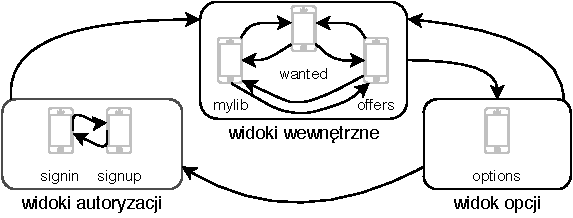
\includegraphics[width=\linewidth]{navig.pdf}
	\caption{\centering Schemat nawigacji pomiędzy ekranami}
	\caption*{\centering Źródło: {Opracowanie własne za pomocą narzędzia \url{https://www.draw.io/}}}
\end{figure}
%---------------------------------------------------------------------------

\section{Logowanie i rejestracja}
Te dwa ekrany zawierają formularze w których użytkownik może wpisać email oraz hasło. Po wpisaniu danych, akceptuje formularz niebieskim przyciskiem i tworzy zapytanie do Auth Service (2.2). W sytuacji, gdy wprowadzone dane są niewłaściwe, zostanie wyświetlony odpowiedni komunikat.
Na dole ekranu widnieje krótki tekst, po którego kliknięciu, nastąpi zresetowanie formularza i przeniesienie do sąsiedniego widoku.

\begin{figure}[H]
	\centering
	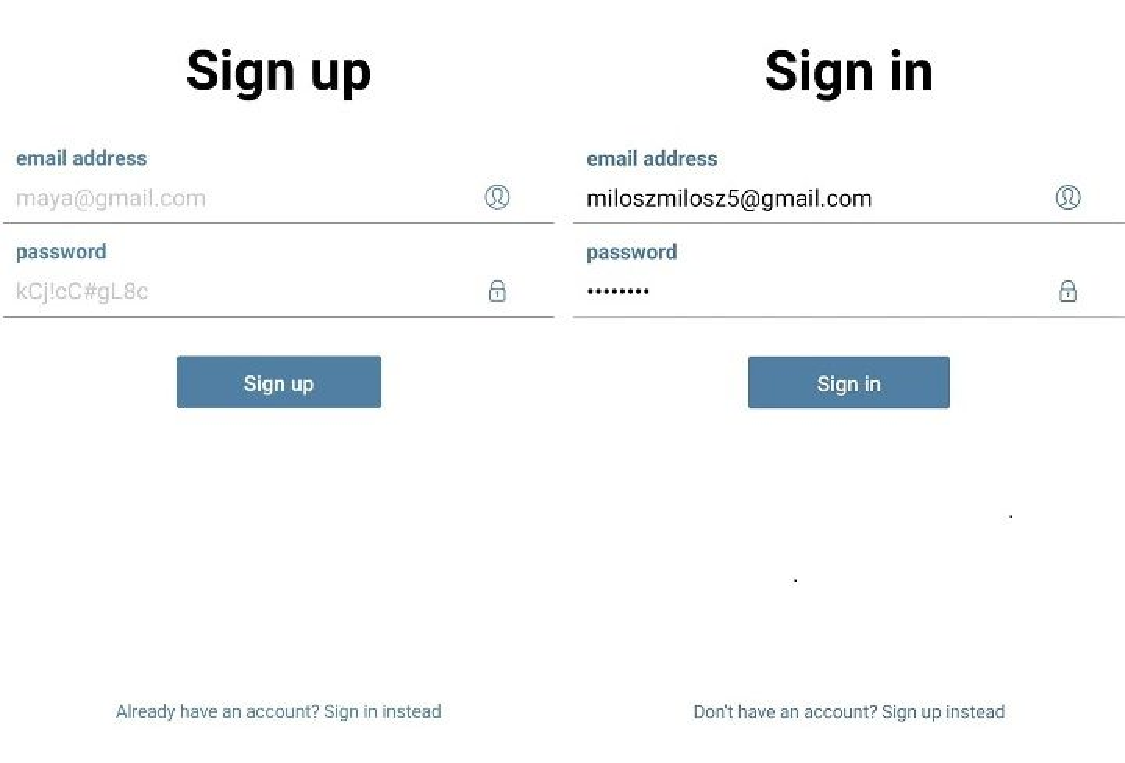
\includegraphics[width=\linewidth]{signin_signup.pdf}
	\caption{\centering Ekrany logowania i rejestracji w aplikacji mobilnej}
	\caption*{\centering Źródło: {Opracowanie własne}}
\end{figure}
%---------------------------------------------------------------------------
\section{Ekrany bibliotek}
Widoki \textit{Wanted} i \textit{My library} korzystają w większości z tych samych komponentów, różni je natomiast sposób oraz cel ich użycia. Obydwa zawierają listy(rodzaj komponentu), których jedynie widoczne elementy są renderowane, aby nie spowalniać pracy aplikacji. Można je przesuwać werykalnie, a każdy element posiada ukryte opcje z lewej i prawej strony, które można aktywować poprzez horyzontalne przesunięcie wykonane na pojedynczym segmencie.


Widok poszukiwanych książek prezentuje pozycje, które będą wysłane do serwisu OffersFetcher (2.4)  i użyte w celu stworzenia ofert.
Na poniższej grafice widnieje funkcjonalność dodawania nowej pozycji do listy. Po naciśnięciu  obszaru z napisem ``new book``, wysunięty zostanie formularz, który poprawnie wypełniony poskutkuje dodaniem nowej książki i wysłaniem jej do bazy danych w chmurze. Cenę każdej pozycji można edytować po jej naciśnięciu - pojawi się pole do edytowania wartości.
\begin{figure}[H]
	\centering
	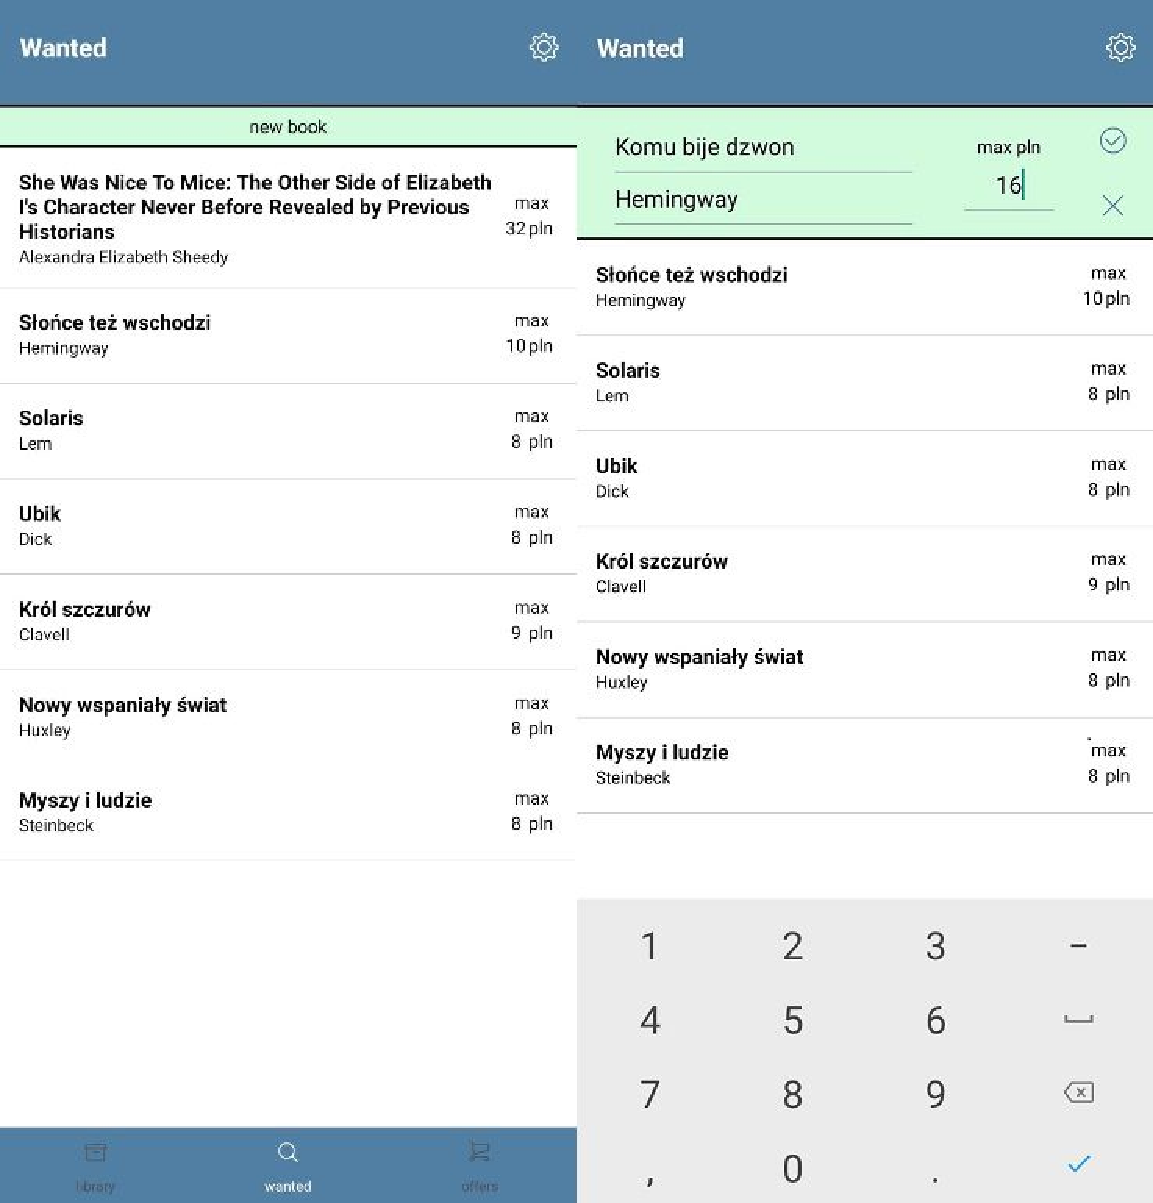
\includegraphics[width=\linewidth]{wanted.pdf}
	\caption{\centering Biblioteka poszukiwanych książek oraz dodawanie nowej pozycji}
	\caption*{\centering Źródło: {Opracowanie własne}}
\end{figure}


Poprzez przesunięcie pojedynczego elementu w lewo, pojawi się ukryty pod spodem przycisk, który służy do usunięcia danej książki z listy i bazy danych. Jeżeli bloczek poruszony zostanie ruchem o przeciwnym zwrocie, użytkownik otrzyma możliwość edytowania informacji o danym tomie.
Każde wychylenie elementu zostanie przywrócone do stanu wyjściowego w momencie poruszenia innej pozycji lub po 5 sekundach bezczynności.
\begin{figure}[H]
	\centering
	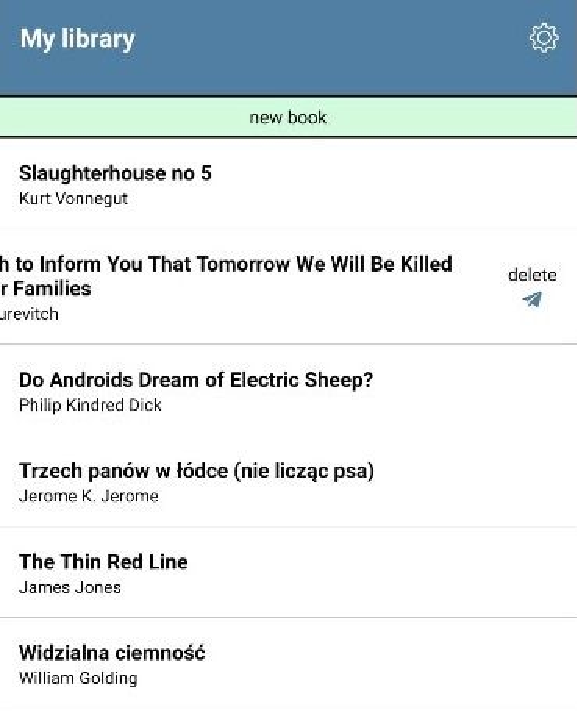
\includegraphics{mylib.pdf}
	\caption{\centering Bilbioteka posiadanych książek oraz funkcjonalność usuwania}
	\caption*{\centering Źródło: {Opracowanie własne}}
\end{figure}

%---------------------------------------------------------------------------

\section{Ekran z ofertami}
To tutaj zaprezentowane są wyniki analiz wykonanych w serwisie OffersFetcher (2.4). Jest to przesuwalny wertykalnie komponent zawierający sprzedawców oraz ich produkty, na bazie pozycji z ekranu Wanted. Każdy element składa się z identyfikatora właściciela aukcji, następnie z listy książek, gdzie każdy obiekt to zdjęcie prezentujące produkt, tytuł, autor, a także jego cenę. Na dole oferty wyświetlona jest sumaryczna cena tomów oraz najtańsza możliwa dostawa według kontrahenta.
\begin{figure}[H]
	\centering
	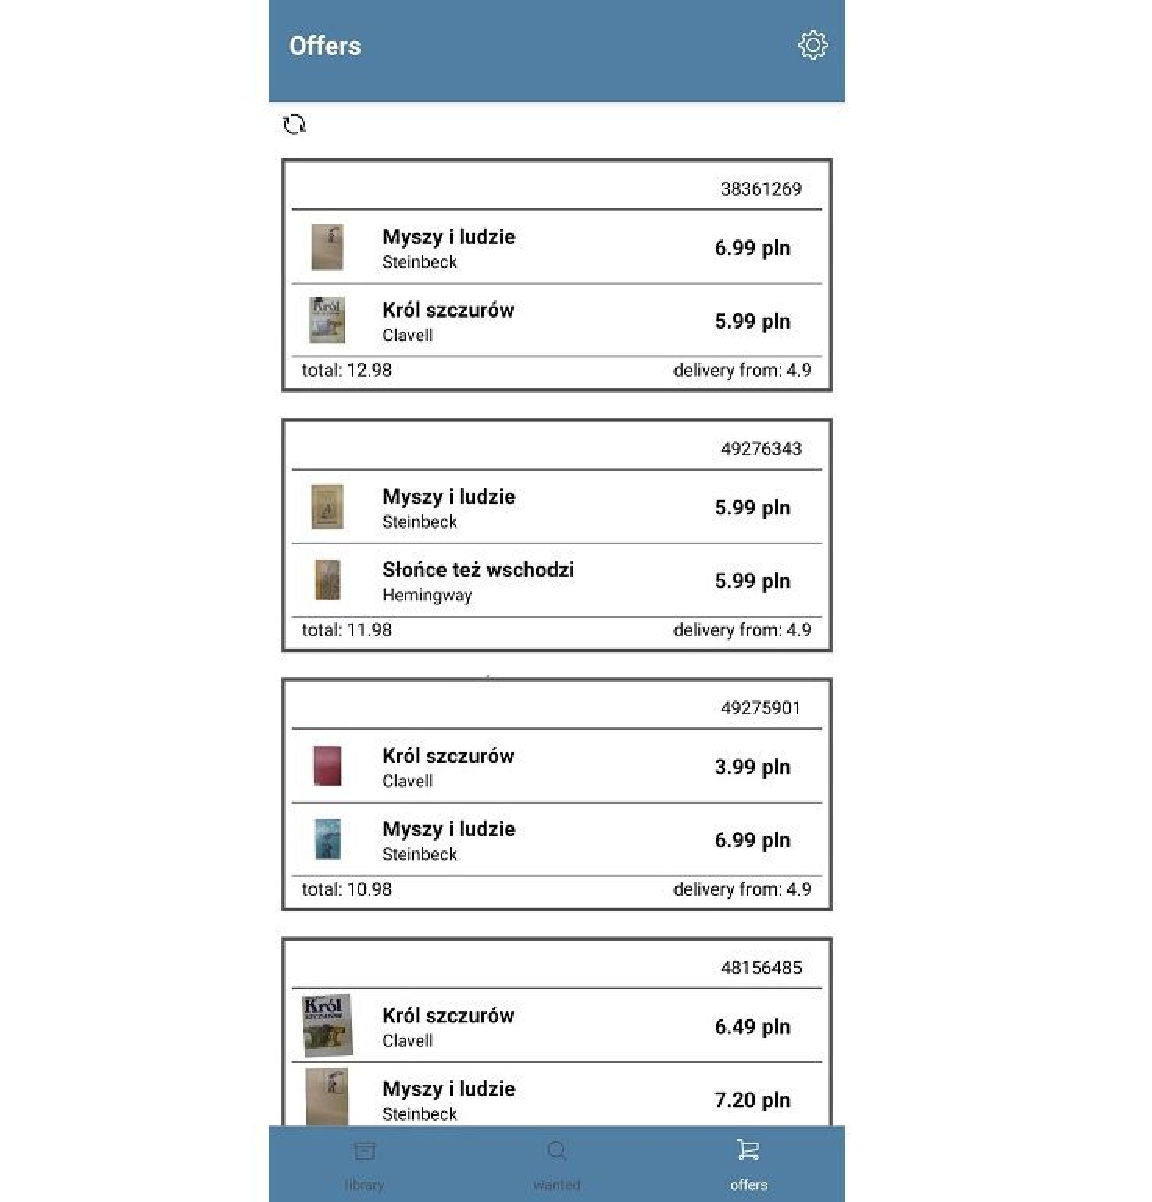
\includegraphics[width=\linewidth]{offers.pdf}
	\caption{\centering Ekran prezentujący oferty od sprzedawców}
	\caption*{\centering Źródło: {Opracowanie własne}}
\end{figure}

\newpage
\section{Opcje}
Obecnie na ekranie opcji, który można wywołać po naciśnięciu przycisku w prawym górnym rogu, dostępna jest tylko jedna opcja - mianowicie wylogowanie użytkownika. Po naciśnięciu przycisku, usunięty zostanie token dostępowy, a aplikacja wykona przeniesienie do ekranu logowania.
\begin{figure}[H]
	\centering
	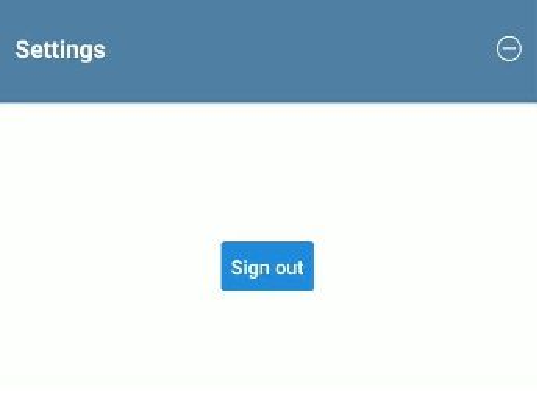
\includegraphics{options.pdf}
	\caption{\centering Ekran opcji z możliwością wylogowania}
	\caption*{\centering Źródło: {Opracowanie własne}}
\end{figure}

